% -*- TeX-master: "../fat_manual.tex" -*-

\newpage\section{System and amplifiers}
  The connections from the top of the system are as follows
  \begin{center}
	  	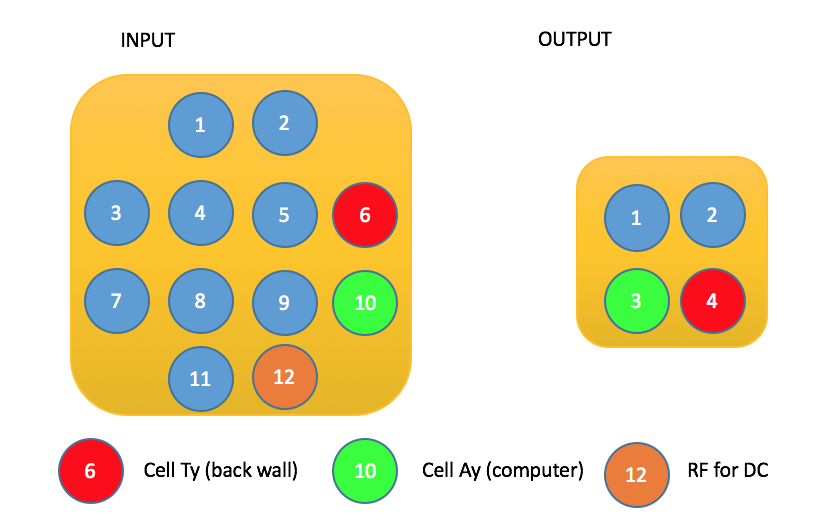
\includegraphics[height=5cm]{top}
	  	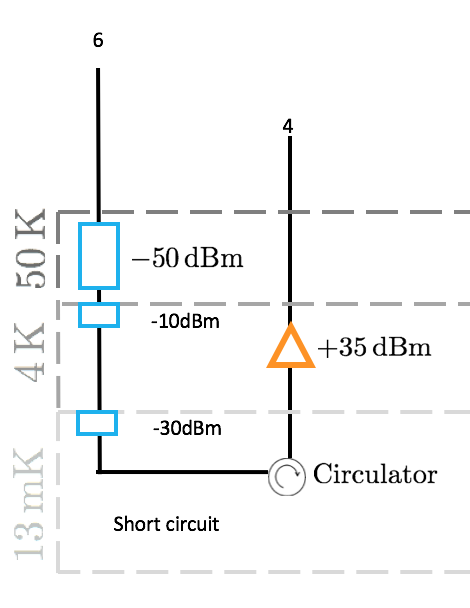
\includegraphics[height=5cm]{side}
  \end{center}
 	
 	The attenuator markings, which are attached to the various plate, have the last number depicting the atuniation. \red{\textbf{Note, that it can be 0dB!!!}}
 	\begin{center}
 		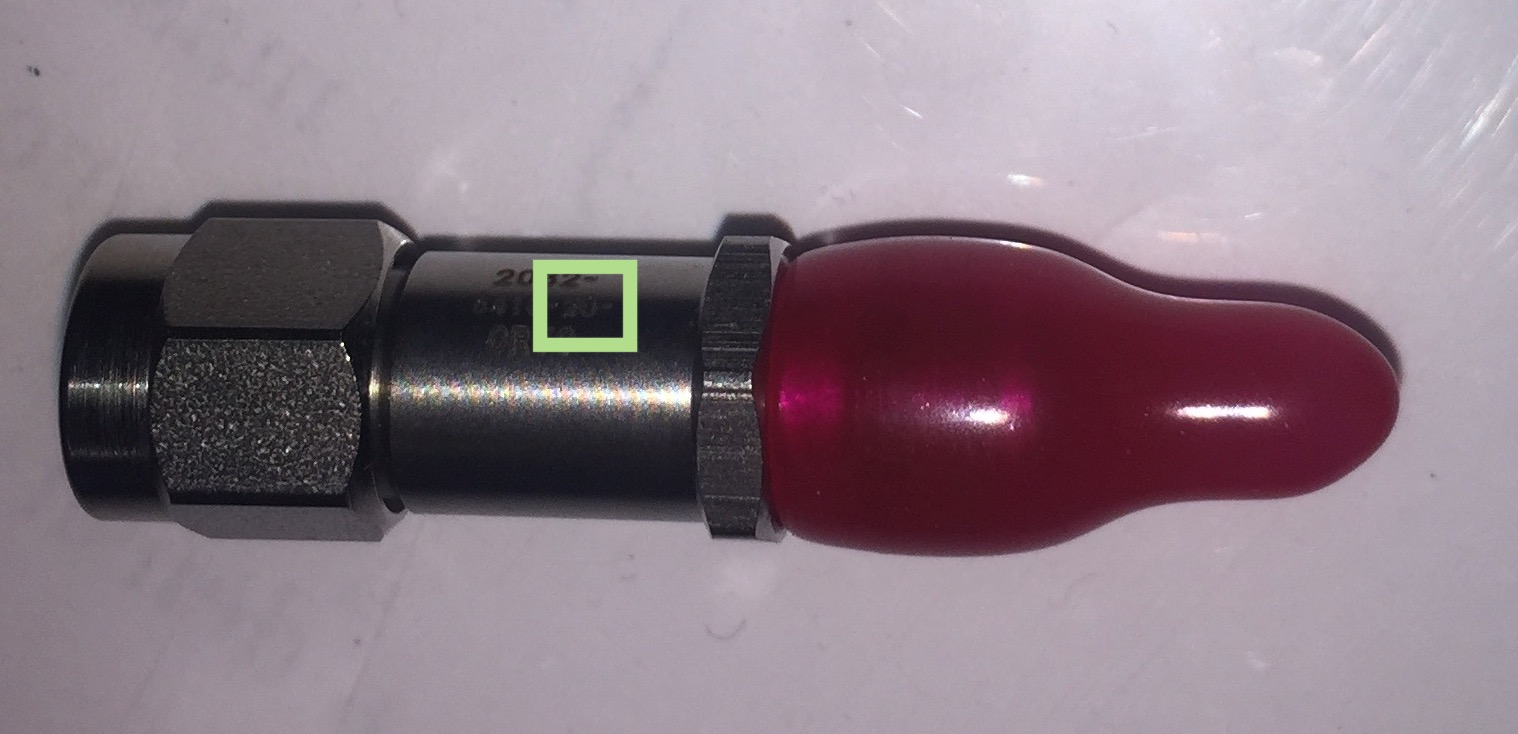
\includegraphics[height=5cm]{filter}
 	\end{center}
 	
 
 \red{\textbf{\Large Turn amplifiers off when handling them!}}
 
  In order to turn both the room temp and cold amplifiers on, we need to apply voltages 
  \begin{enumerate}
  	\item \href{http://www.lownoisefactory.com/products/roomtemp/1-15-ghz/}{\textbf{LNF-LNR1\_15A}} Climb up on the ladder \ra turn the power supply on \ra turn the small \mi{on} buttons at the bottom of the amplifier to \mi{on} at the same time; 
  	\[
  		\text{Left display:} 2.44V \quad \text{Right display:}2.67\,\text{V}
  	\]
  	\item There are two {LNF-LNR1\_15A} amplifiers:
  	\begin{itemize}
  		\item Input 10, Output 3, Cell Ay, 337\,V, closer to computer;
  		\item Input 6, Output 4, Cell Ty, 330V, closer to back wall;
  	\end{itemize}
  	On each line there is a 50dB attenuator in the top hood, 10dBm on the 4K plate (first grey plate), 30dB on the 13mK plate.
  	Turn on the correct switch on the grey box;
  	\item My \href{http://www.atlantecrf.com/products/active_components/amplifiers/wide_band_amplifiers.htm}{AOX-010120 amplifier} just needs 5\,V from any supply.
  \end{enumerate}
  \newpage
  
 \section{DC PCB}
  The DC samples are connected as in the figure below:
  \begin{itemize}
  	\item {\LARGE \red{In the designs, the RF lines and GROUND are on the LEFT-HAND SIDE, and therfore the chips need to be flipped so that RF is on the RIGHT!}}
  	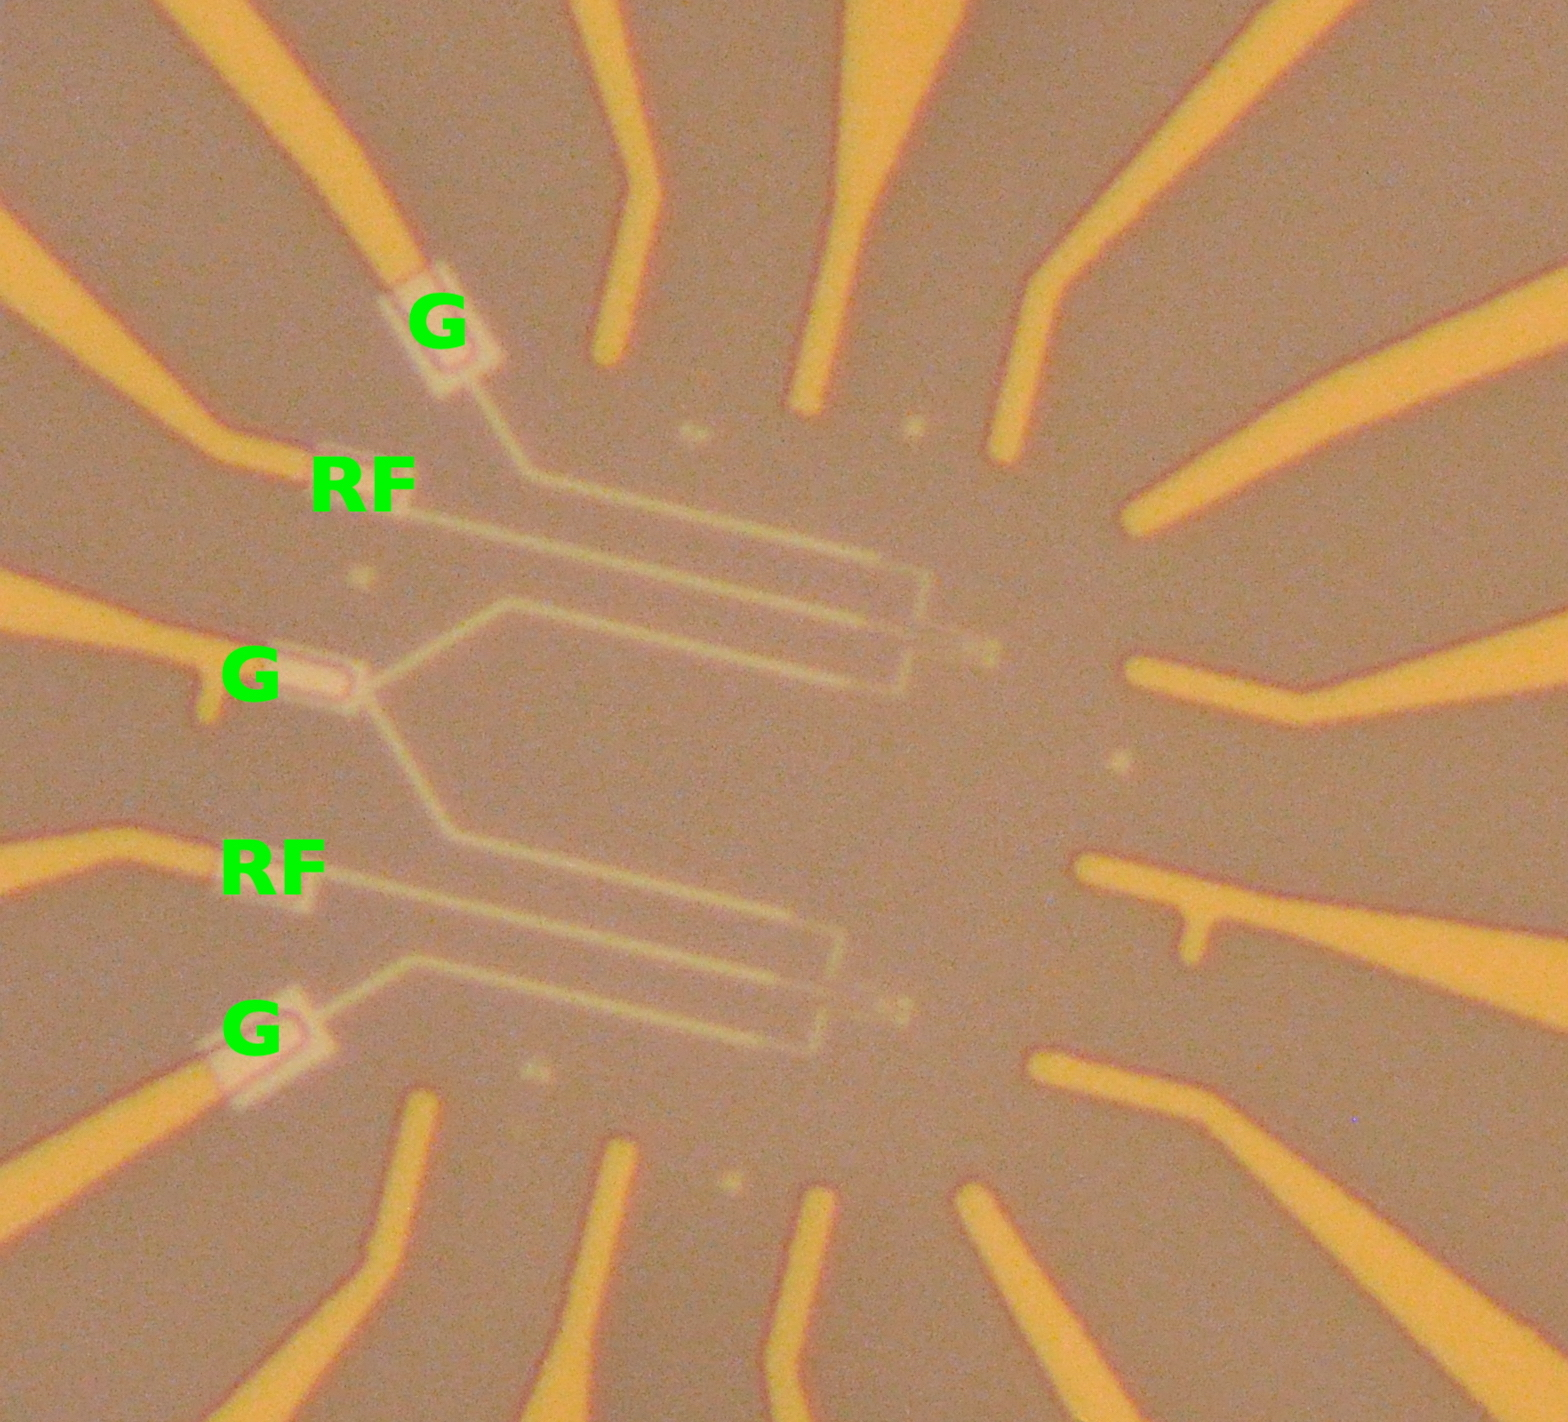
\includegraphics[height=2cm]{F}
  	\item The RF bias is on the RHS of the PCB;
  	\item Numeration of contacts on the PCB begin below the RF line and goes clockwise;
  	\item Position 2 is on top, Position 1 is on bottom (remember to flip the chips);
  	\item \red{Attach with small drop of resin \textbf{so that chip 1 and chip 2 are exposed to contacts 1,2,3,4};}
  	\item \red{Remove with scalpel and wash chips in acetone.}
  \end{itemize}
 
 \begin{figure}[h]
 	\centering
 	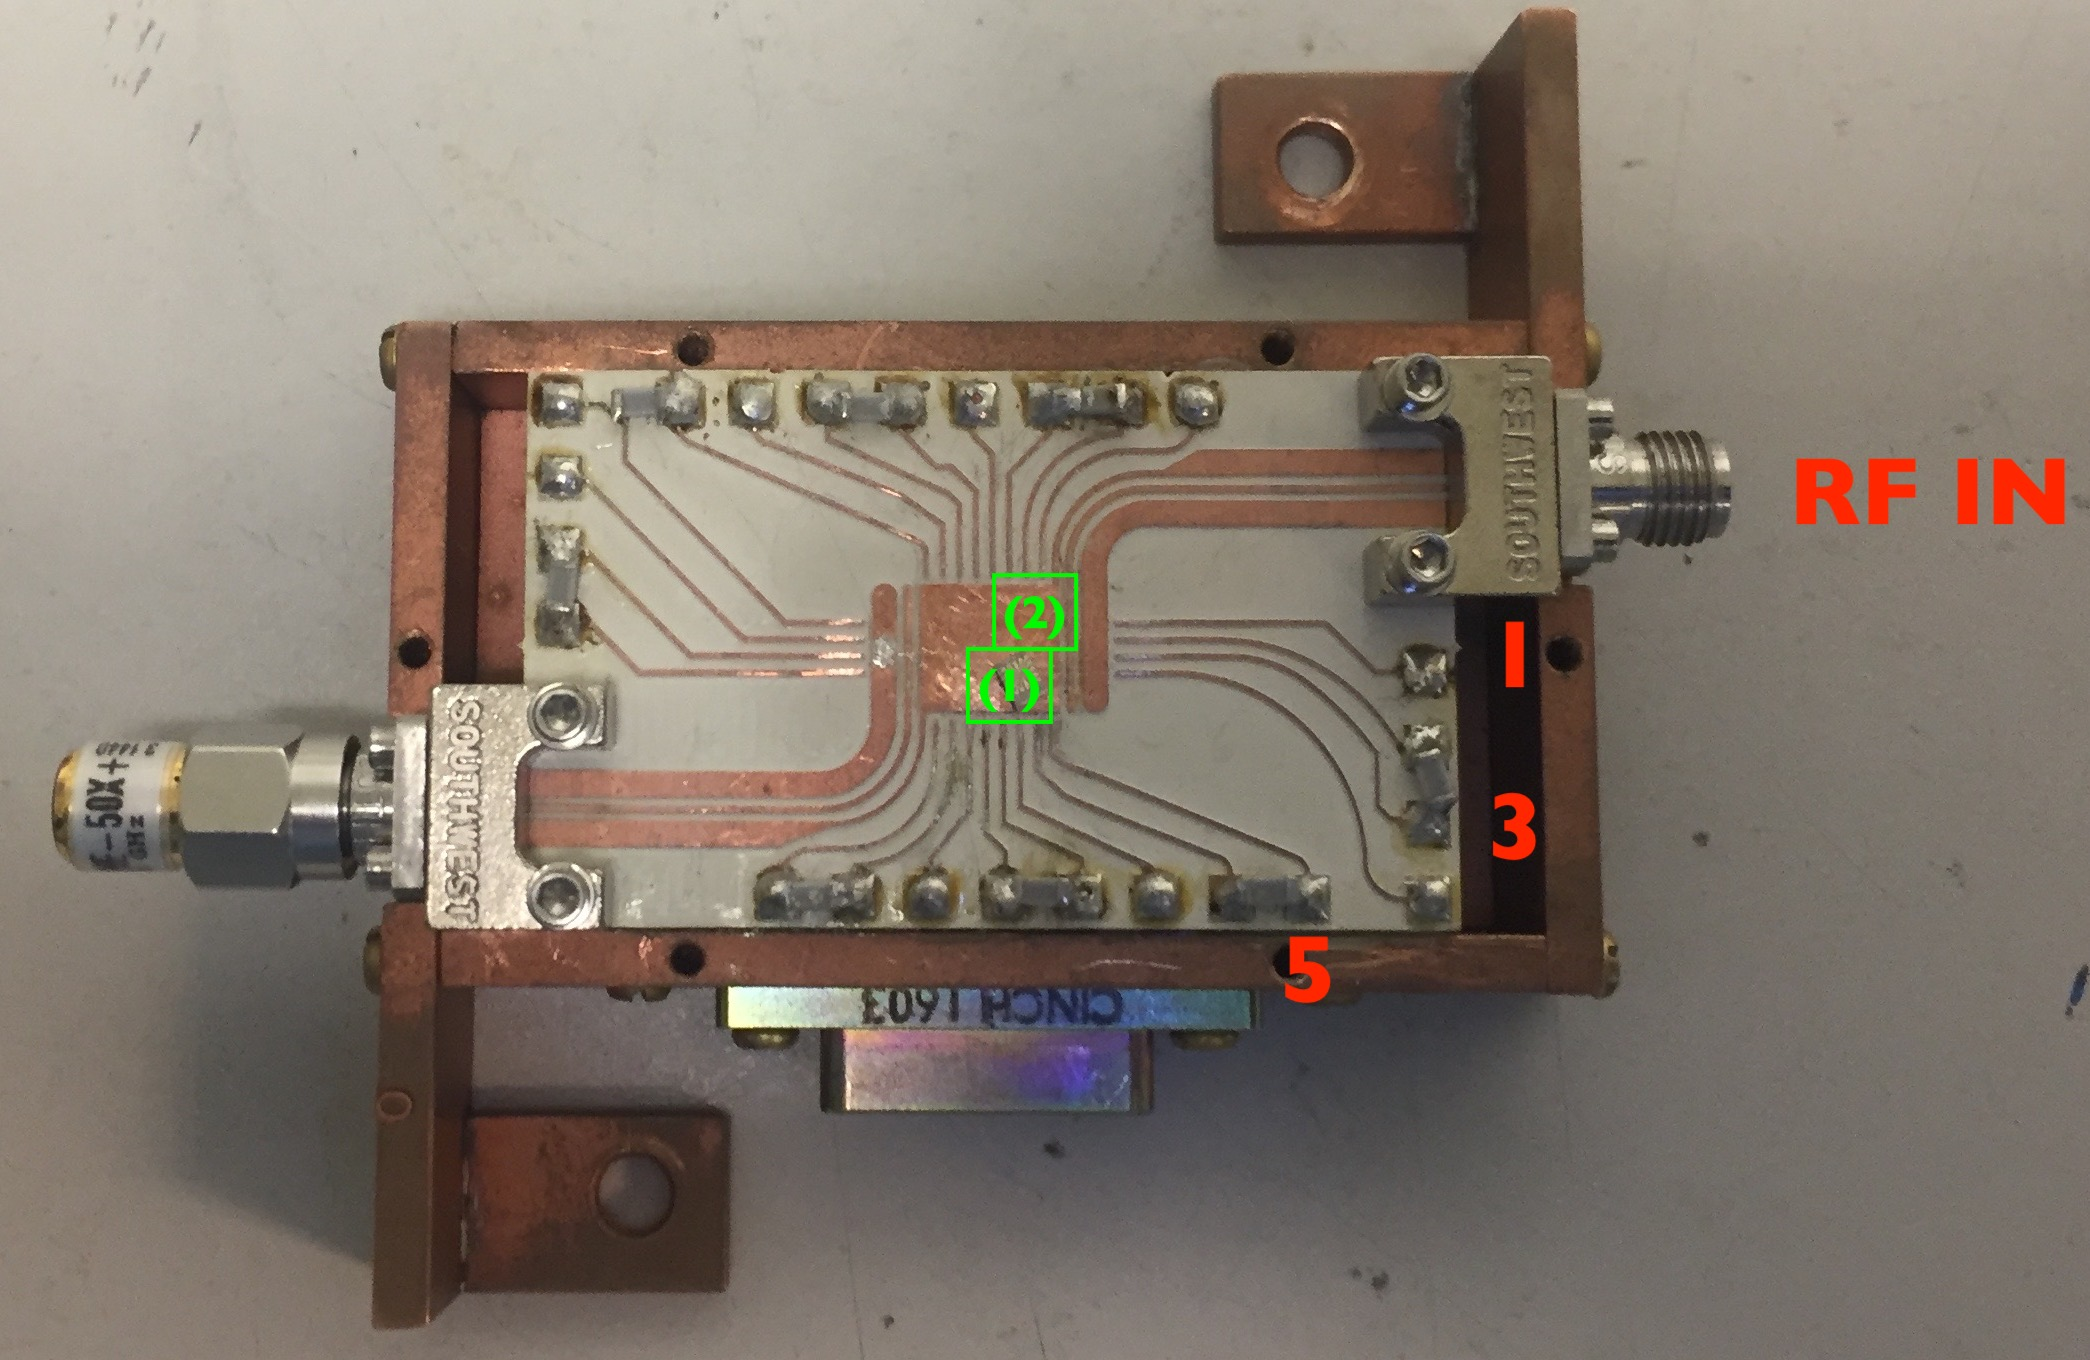
\includegraphics[height=7cm]{pcb1}
 	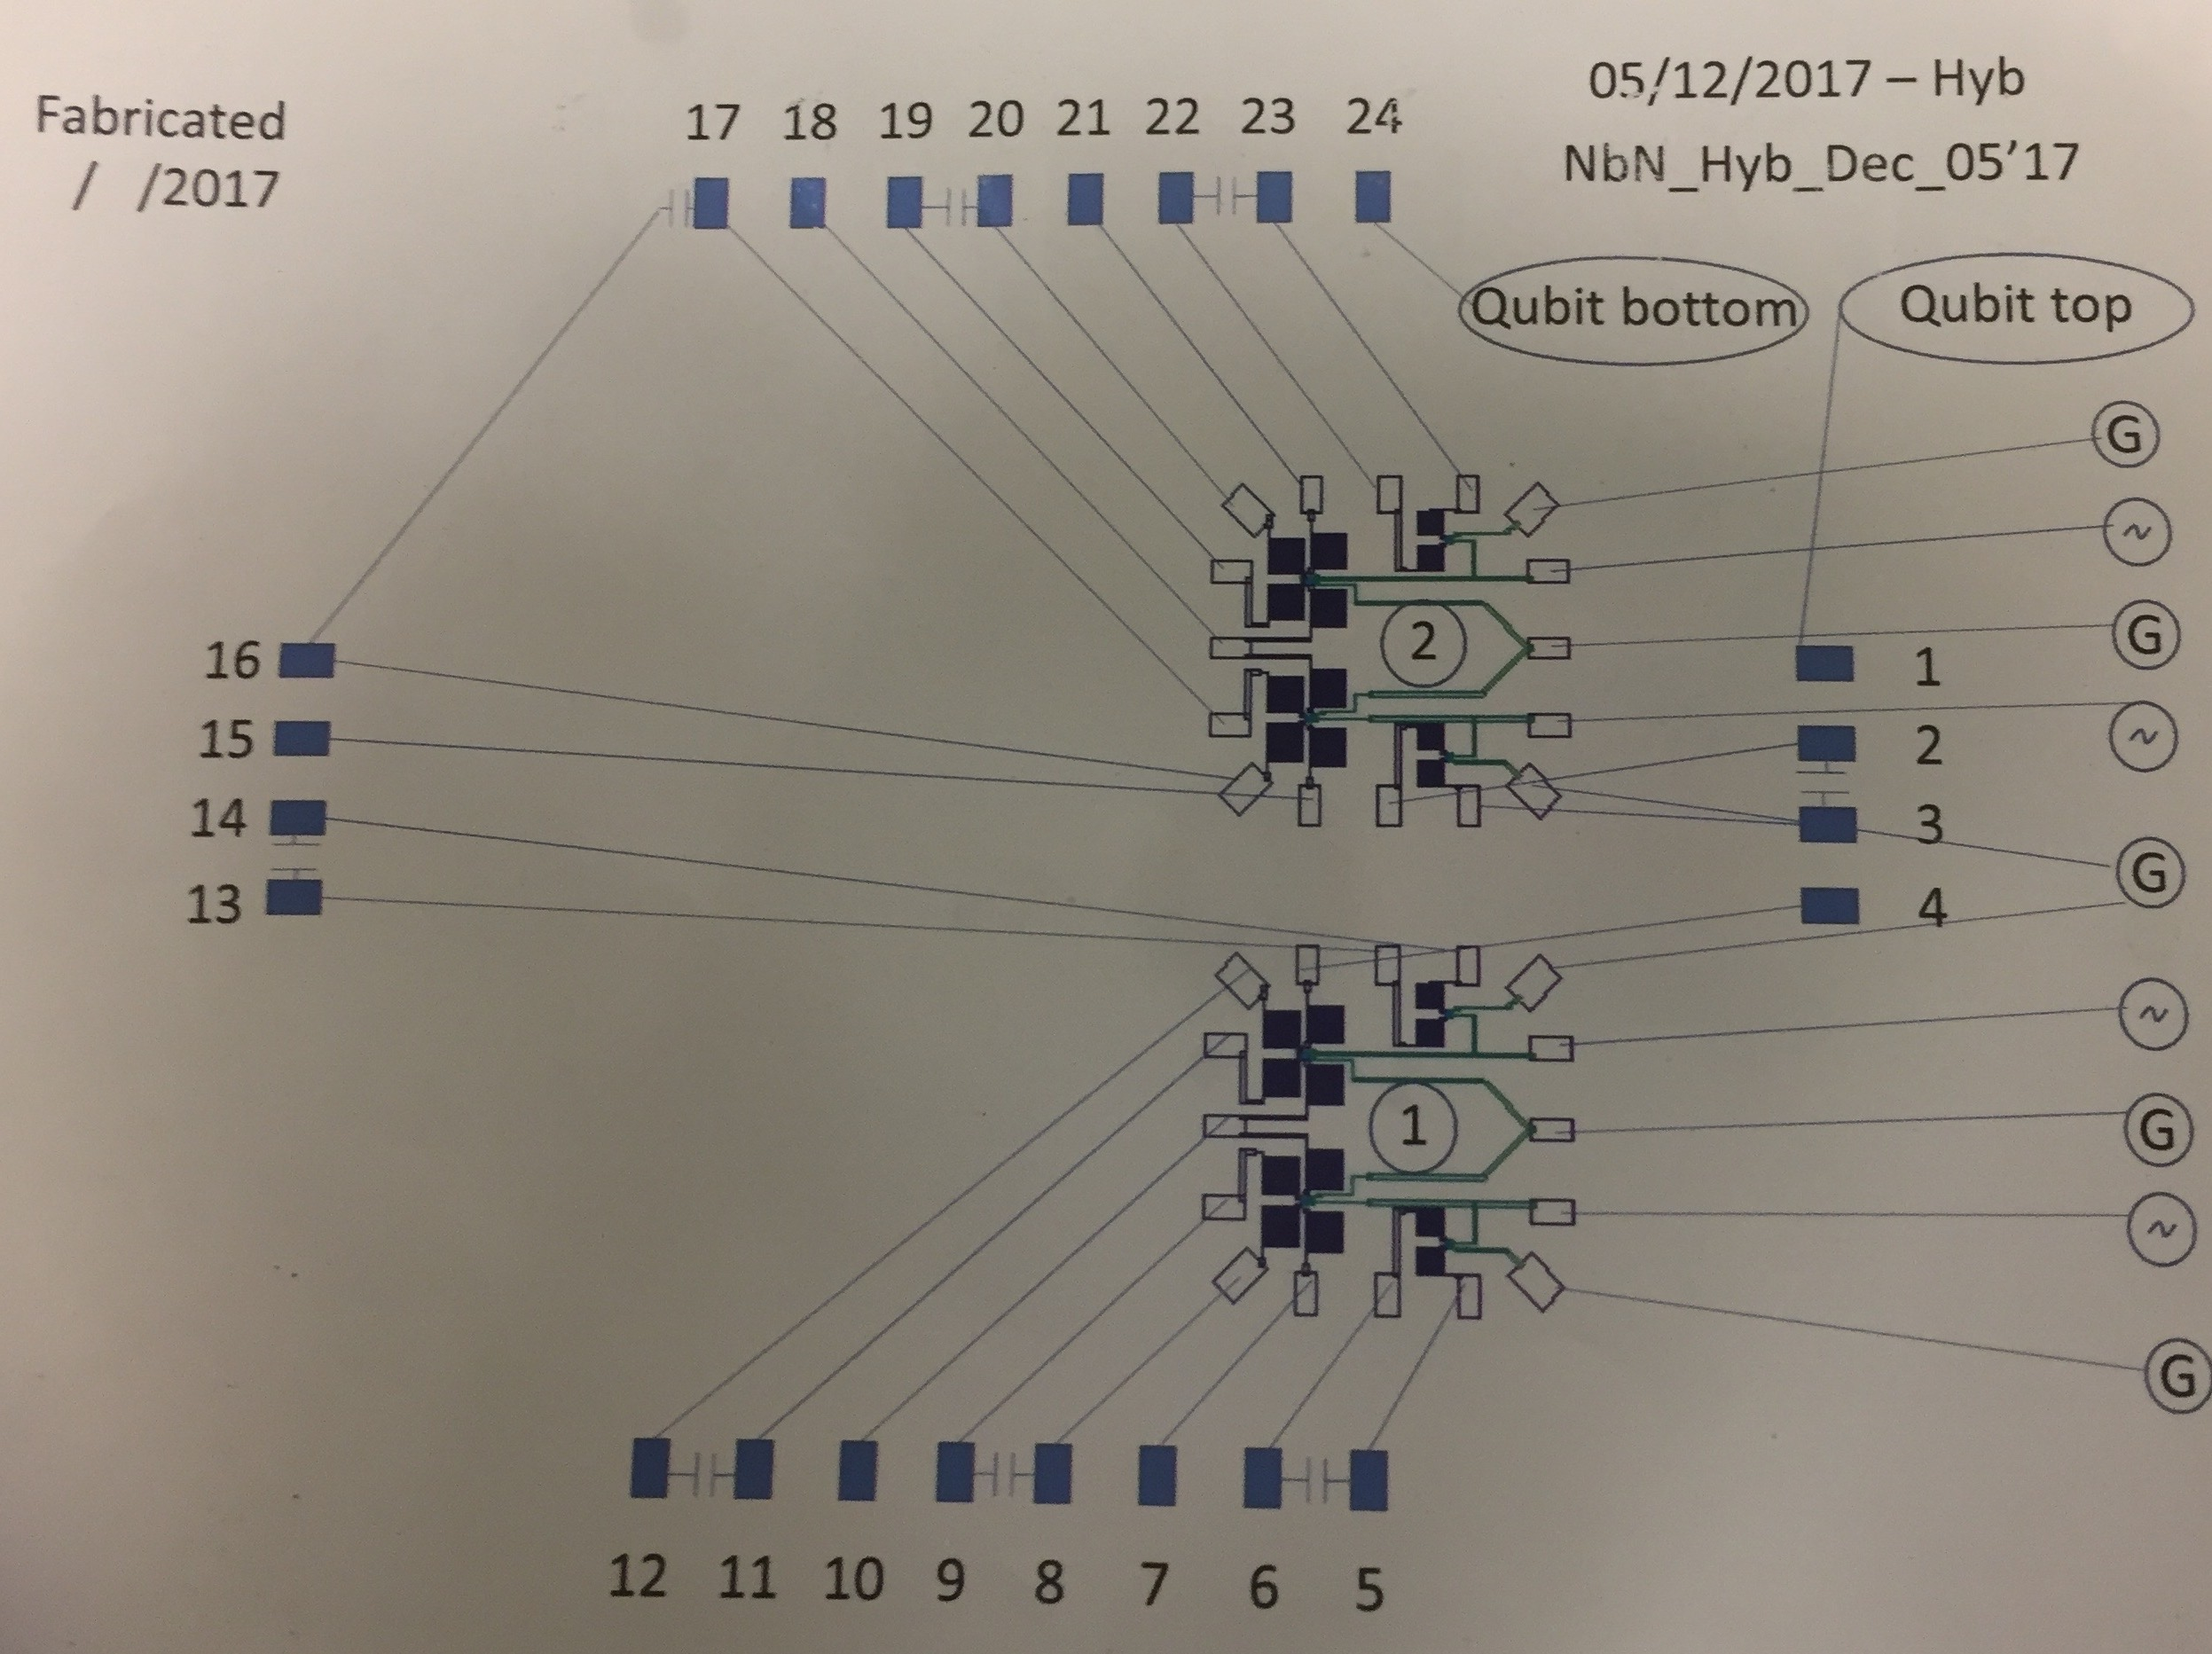
\includegraphics[height=7cm]{pcb2}
 \end{figure}
 \newpage 
 
 \section{Ethernet}
  Devices are connected via one breakout ethernet box to computers with DNS name 196.168.0.64
  \begin{itemize}
  	\item VNA 196.168.0.3
  	\item Blueforce 192.168.0.4
  	\item PC Rais 192.168.0.2
 	\item SPA 192.168.0.6
 	\item My one 192.168.0.1
 	\item Generator 192.168.0.7 
 	\item Pulse generator 192.168.0.8	
  \end{itemize}
 
 
\newpage
 
 \section{Adding gate voltage to qubits}
For some experiments we add a gate voltage to the system. The circuit for this setup is the following:

\begin{center}
	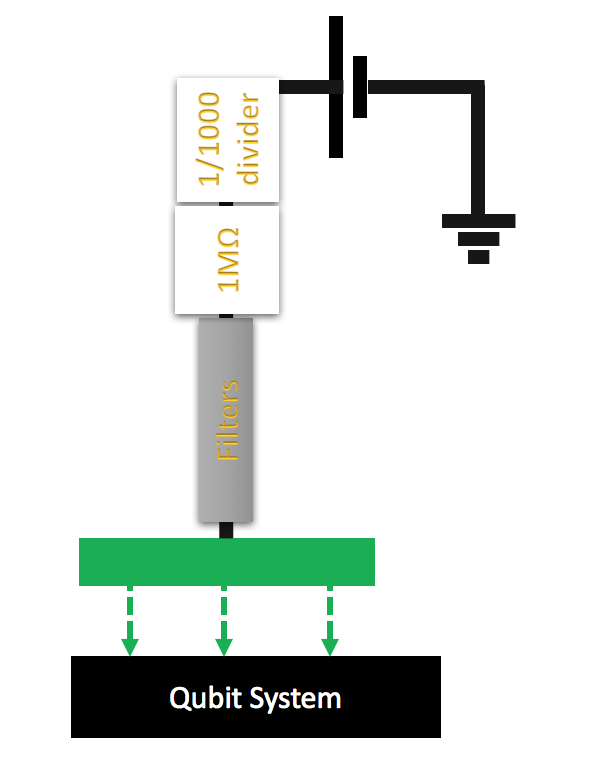
\includegraphics[height=7cm]{gate}
\end{center}

The resistor is there to damped any noise. The voltage $ \approx 5\, $V is then felt by the qubit system across from the gate electrode.

\newpage 